\section{Auswertung}
\label{sec:Auswertung}

\begin{table}
  \centering
  \caption{Aufgenomme Werte }
  \label{tab:werte}
  \sisetup{round-mode = places , round-precision = 2}
  \begin{tabular}{S S S S S S}
    \toprule
    {$t/\si{\minute}$} & {$T_1/\si{\celsius}$} & {$T_2/\si{\celsius}$} & {$p_A/\si{\bar}$} & {$p_B/\si{\bar}$} & {$P/\si{\watt}$} \\
    \midrule
    1         & 20.6 & 19.9 & 2.4  & 6.5   &  170\\
    2         & 21.6 & 19.8 & 2.6  & 7.0     &  178\\
    3         & 22.9 & 18.9 & 3.0    & 7.25  &  185\\
    4         & 24.6 & 17.4 & 3.0    & 7.5    & 195\\
    5         & 26.5 & 15.6 & 3.2  & 8.0     &  200\\
    6         & 28.6 & 13.7 & 3.2  & 8.5     &205\\
    7         & 30.5 & 11.9 & 3.2  & 8.75   & 205\\
    8         & 32.6  &9.9  & 3.2  & 9.25   & 207\\
    9         & 34.5 & 8.0  & 3.2  & 9.5    & 210\\
    10        & 36.5 & 6.3  & 3.2  & 10.0     & 208\\
    11        & 38.4 & 4.4  & 3.2  & 10.5   & 210\\
    12        & 40   & 3.0  & 3.2  & 10.75  & 213\\
    13        & 41.7 & 1.9   &3.2  & 11.25  & 213\\
    14        & 43.3 & 1.0  & 3.2  & 11.5   & 210\\
    15        & 44.9 & 0.4  & 3.2  & 12.0     & 208\\
    16        & 46.3 & -0.2 & 3.2  & 12.25  & 205\\
    17        & 47.6 & -0.7 & 3.2  & 12.5   & 205\\
    18        & 48.7 & -1.1 & 3.2  & 12.75  & 202\\
    19        & 49.9 & -1.6 & 3.2  & 13.0     & 201\\
    20        & 50.9 & -1.9 & 3.25 & 13.5   & 200\\
    \bottomrule
  \end{tabular}
\end{table}

Sämtliche in diesem Versuch aufgenommenen Werte lassen sich Tabelle \ref{tab:werte} entnehmen. Die Temperaturverläufe sind des Weiteren in Abb. \ref{fig:temp} dargestellt, wobei als Fit-Funktion
\begin{equation}
  T(t) = \frac{At^\alpha}{1+Bt^\alpha} +C
\end{equation}
gewählt wurde und $T_2$ lediglich bis Minute $15$ gefittet wurde.
Die Fit-Parameter für $T_1$ ergeben sich so zu:
\begin{align*}
  A_1 &= (-5468 \pm 111) \si{\celsius} \si{\minute}^{1.73} \\
  B_1 &= (110 \pm 3) \si{\minute}^{1.73} \\
  C_1 &= (79.95 \pm 0.66) \si{\celsius} \\
  \alpha_1 & = -1.73 \pm 0.02
\end{align*}
Für $T_2$ gilt entsprechend:
\begin{align*}
  A_2 &= (-0.09 \pm 0.02) \si{\celsius} \si{\minute}^{2.53} \\
  B_2 &= (0.003 \pm 0.006) \si{\minute}^{2.53} \\
  C_2 &= (20.13 \pm 0.15) \si{\celsius} \\
  \alpha_2 & = -2.53 \pm 0.10
\end{align*}

$\frac{\symup{dT}}{\symup{dt}}$ ist durch
\begin{equation}
  \frac{\symup{dT}}{\symup{dt}} = \frac{\alpha At^{\alpha-1}}{\left(1+Bt^\alpha \right)^2}
\end{equation}
gegeben.
\begin{figure}
  \centering
  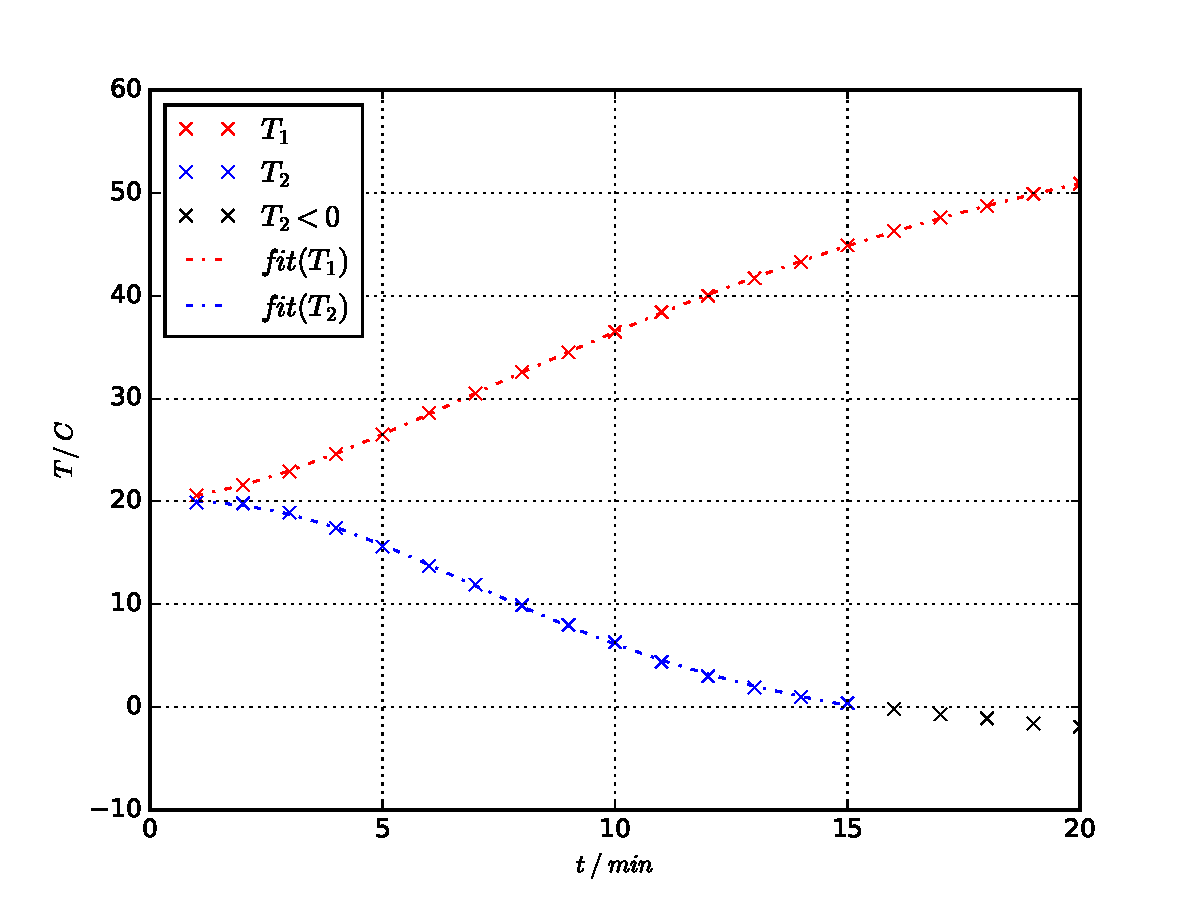
\includegraphics[width = \textwidth]{./Plots/Temperaturverlauf.pdf}
  \caption{Verlauf der Temperaturen $T_1$ und $T_2$ sowie Fits.}
  \label{fig:temp}
\end{figure}
